\section{Implementierung}

\begin{figure}[h]
 \centering
 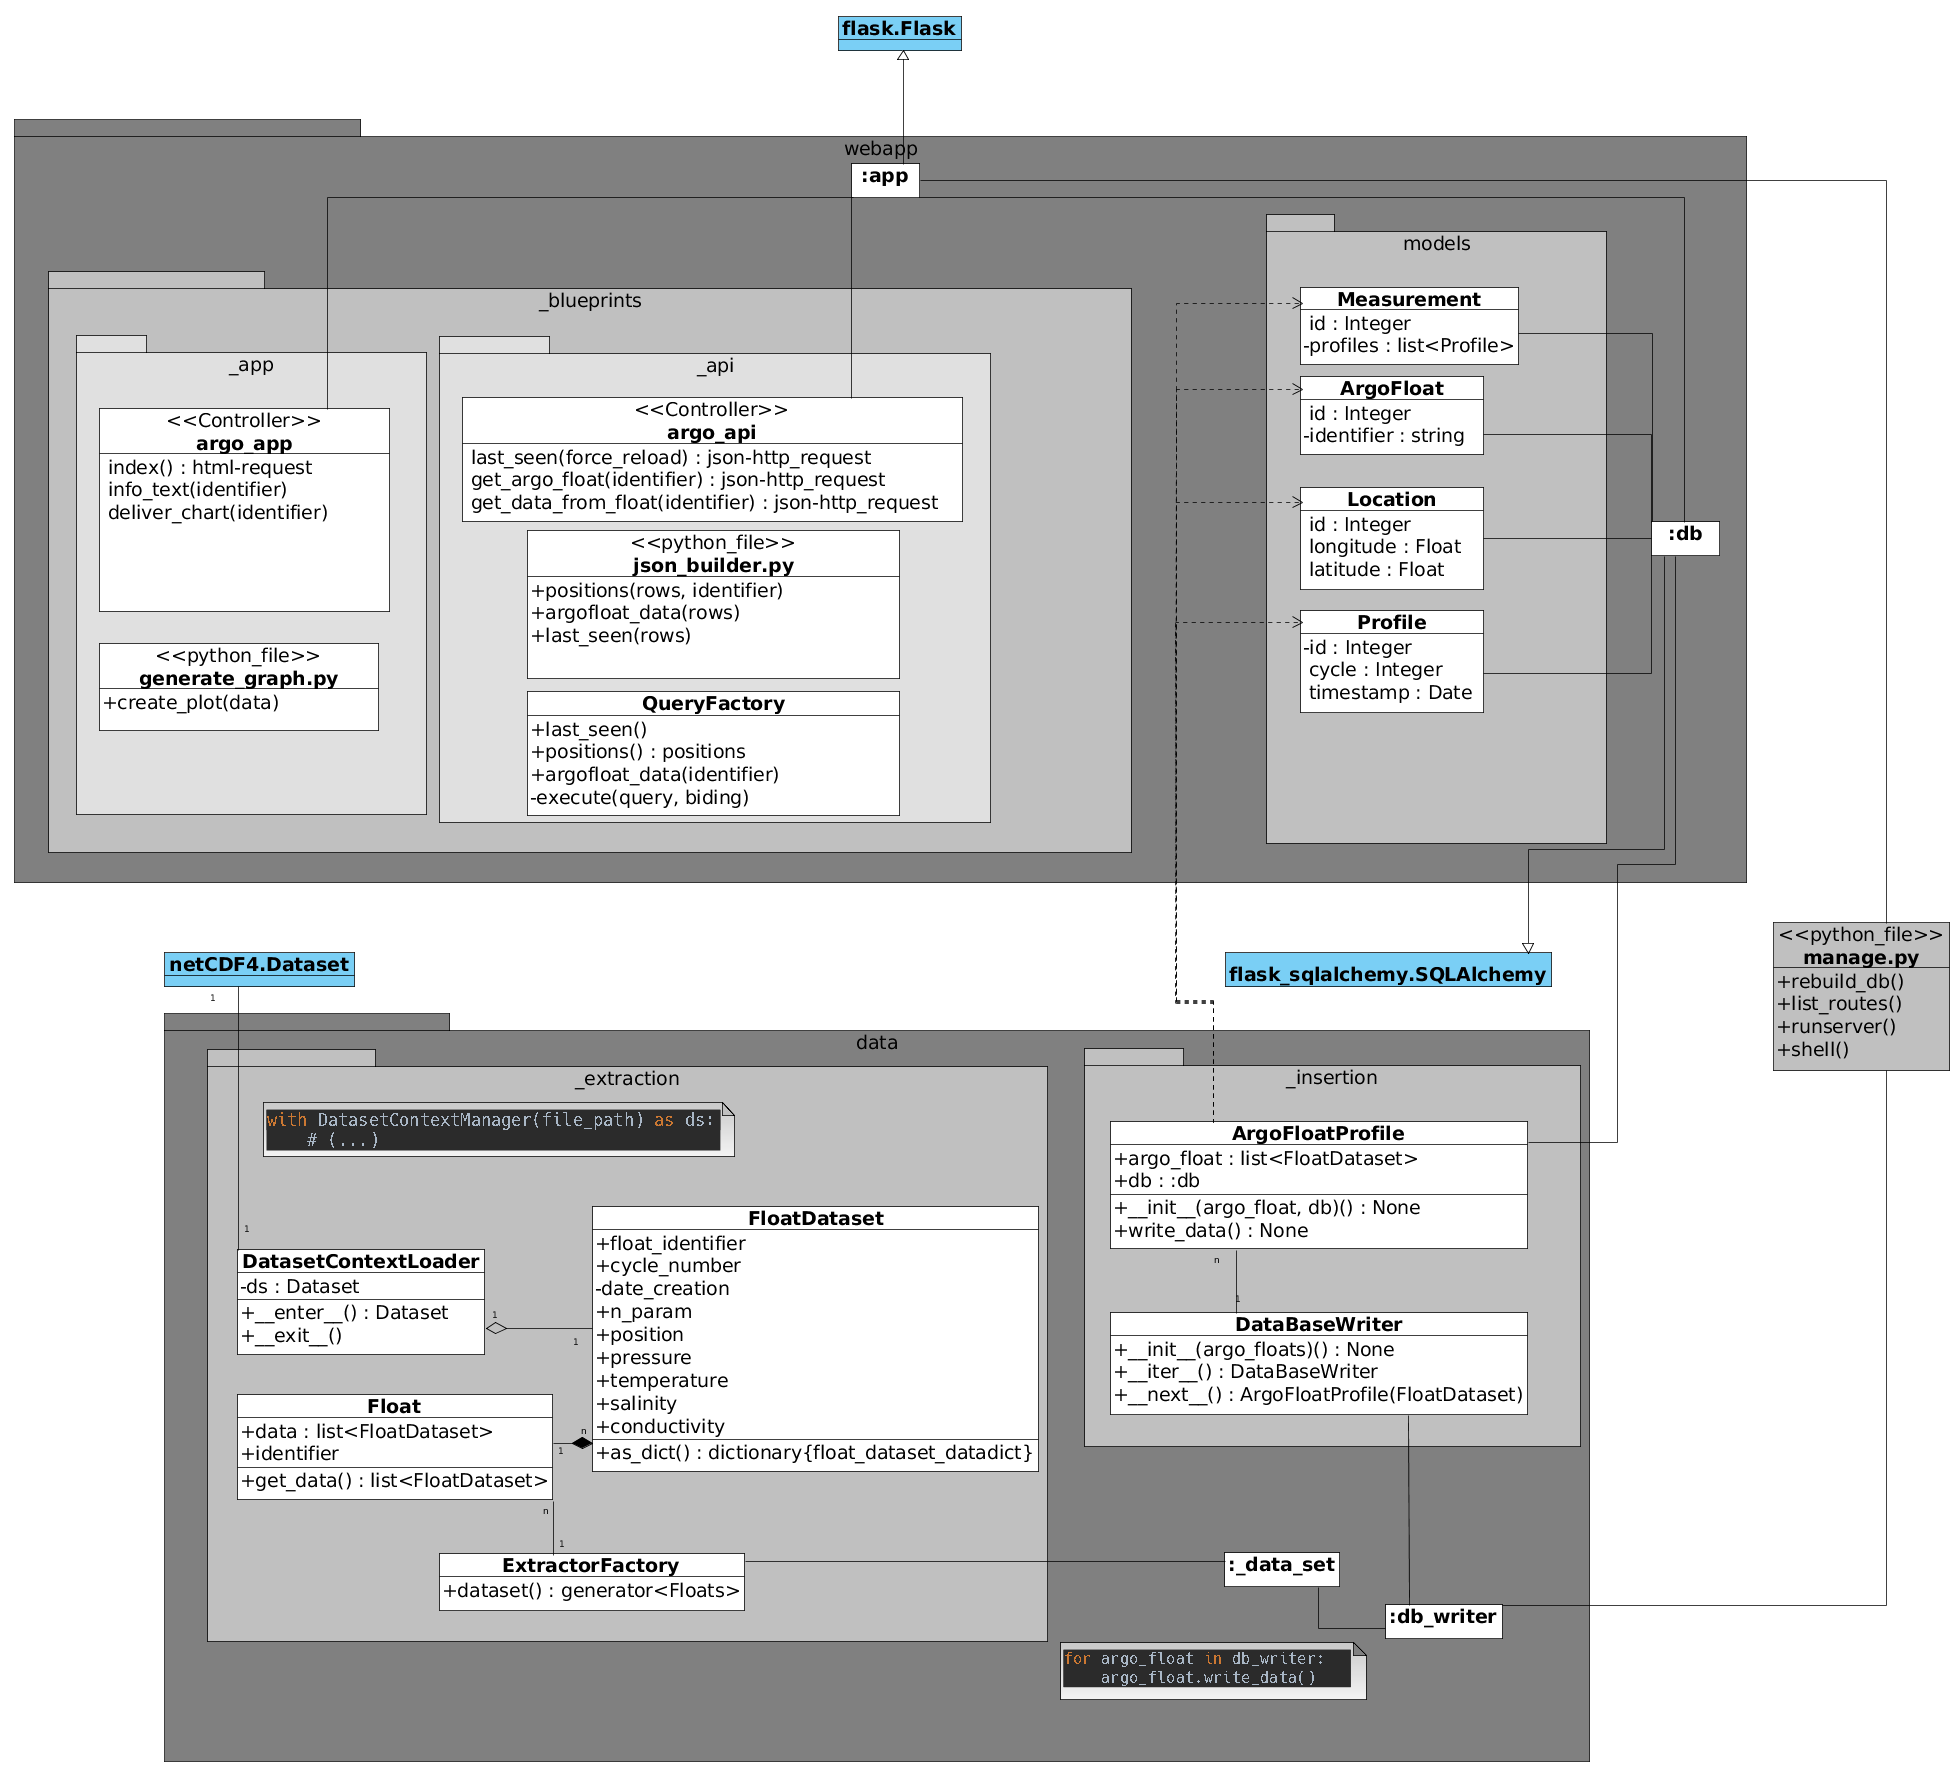
\includegraphics[width=\textwidth]{pix/Modulschema_komplett.png}
 % Modulschema_komplett.png: 876x911 px, 96dpi, 23.17x24.10 cm, bb=0 0 657 683
 \caption{Architekturbeschreibung}
 \label{fig:modulschema}
\end{figure}

% BEGIN DATENAGGREGATION
\subsection{Schnittstellen der Datenaggregation}

Bei der Aggregation der Daten aus dem Argo Programm sind Schnittstellen auszuarbeiten. Diese Implementierung ist im folgenden beschrieben. 

\paragraph{Dateninput}

Der Datensatz besteht vor der Verarbeitung aus zahlreichen Dateien. Da die Gefahr besteht, dass geöffnete Dateien nicht wieder ordnungsgemäß geschlossen werden, muss eine Schnittstelle geschaffen werden, die unsachgemäße Verwendung der Dateien verhindert. 

Python sieht für diesen Zweck den Kontextmanager vor.

\pythonexternal[%
        caption={Implementierung des Kontextmanagers zur Sicherstellung der richtigen Dateibehandlung.}%
        label=lst:iteratorimpl]{./scr/beispiele/contextmanager.py}



\paragraph{Steuerung}

Um die Verarbeitung der Daten sowie den Prozess der Aggregation in der Datenbank richtig zu modellieren, ist es sinnvoll, den Prozess als Sequenz zu modellieren. Dies erlaubt es, die Datenstruktur über einen Generator vorzuhalten. Python sieht dafür den Iterator vor.

Die hier verwendete Implementierung ist in Listing \ref{lst:iteratorimpl} zu sehen. Das Interface wird über die Funktion \pythoninline{def __next__(self)} in Zeile 12 realisiert. 
Dieses delegiert die Iteration zum Objekteigenen Generator \pythoninline{self.argo_floats}. In dem Moment, in dem ein Objekt aus dem Generator verarbeitet wird, findet die Verarbeitung der dem zugrunde liegenden Datenstruktur statt.

In Zeile 14 wird der Datensatz über ein Objekt ausgeliefert, dass es erlaubt, die Daten in die Datenbank zu überführen.

Damit ist sichergestellt, dass der Prozess nur als Sequenz verwendet werden kann.

\pythonexternal[%
        caption={Implementierung des Iterators zur Steuerung der Aggregationssequenz}%
        label=lst:iteratorimpl]{../BA_argo_proto/data/_insertion/_database_writer.py}

Die Verwendung der Schnittstelle ist in Listing \ref{lst:iterator_verwendung} zu sehen. Dabei wird die Sequenz in Zeile 3 iteriert um den Datensatz daraufhin über die daraufhin folgende Zeile in die Datenbank zu überführen.

\pythonexternal[%
        caption={Verwendung der Schnittstelle zur Steuerung der Datenaggregation}%
        label = lst:iterator_verwendung]{./scr/beispiele/lst-iterator-verwendung.py}
    
    
    
\paragraph{Die Extraktion der Daten über Lazy Loading} ist eine zentrale Problemstellung des Programmablaufs an dieser Stelle. Aus diesem Grund wurde eine Factory Klasse implementiert um den Vorgang und die Datenstruktur in einem generator-Objekt zu realisieren. Der Vorteil eines Generators gegenüber einer Liste Oder Tupes besteht darin, dass Daten erst zu dem Zeitpunkt angefragt und geschaffen werden, wenn diese aus der Sequenz angefordert werden. In Listing \ref{lst:dataextractor} ist die Implementierung dieser Schnittstelle zu sehen. Diese erwartet als Parameter den Pfad zum Verzeichnis, der netCDF-Daten. 

Die Methode \texttt{get\_data\_sets()} erzeugt aus jedem Unterordner im definierten Arbeitsverzeichnis ein Float-Objekt und gibt dieses über das Schlüsselwort \texttt{yield} zurück. 

Durch diese Klasse wird somit ein Generator definiert, der es erlaubt, alle im Arbeitsverzeichnis definierten ArgoFloat Datenobjekte bereitzustellen, ohne diese bereits bei der Instantiierung kennen und abarbeiten zu müssen.


\pythonexternal[%
        caption = {Factory zur Extrahierung der Datensätze.},%
        label = {lst:dataextractor}
    ]{/home/sebsch/Dokumente/Uni-Workdir/Bachelorarbeit/BA_argo_proto/data/_extraction/_data_extractor.py}

%END

% BEGIN SQLALCHEMY
\subsection{SQLAlchemy}

Die Einbindung von SQLAlchemy in den Kontext der Webapplikation muss Festgelegten Muster folgen. In Abbildung \ref{fig:sequenzSQLALCHEMY} kann dieser Ablauf über ein Sequenzdiagramm nachvollzogen werden.

\begin{figure}[!h]
 \centering
 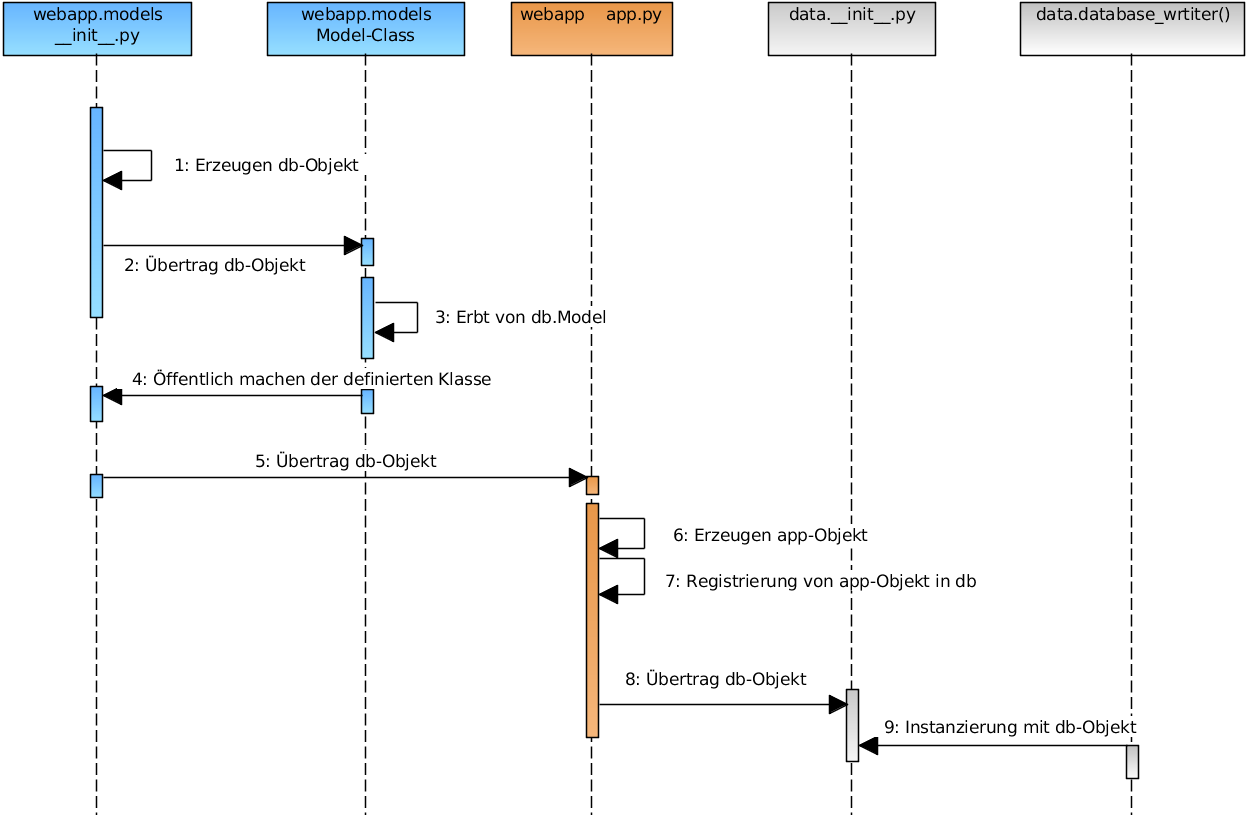
\includegraphics[width=\textwidth]{pix/seq_db.png}
 % seq_db.png: 1310x617 px, 96dpi, 34.66x16.32 cm, bb=0 0 982 463
 \label{fig:sequenzSQLALCHEMY}
\end{figure}

Die Besonderheit in diesem Prozess besteht darin, das zirkuläre Imports vermieden werden müssen. Daher wird das Objekt für die Verwaltung der Datenbank Schritt für Schritt implementiert.

Das Objekt von SQLAlchemy wird bei der Erstellung der Models mit erzeugt.
In Listing \ref{lst:initpy_models} ist dargestellt, auf welche Art die Initialisierung des Moduls \textit{Models} erfolgen kann. 

\pythonexternal[%
    caption={Initialisierung der Mpodulstruktur mitsamt SQLAlchemy},%
    label={lst:initpy_models}]{/home/sebsch/Dokumente/Uni-Workdir/Bachelorarbeit/BA_argo_proto/webapp/models/__init__.py}
    
Die Schnittstelle zur Datenbank wird in Zeile 3 über eine Instanz der Klasse SQLAlchemy initialisiert. Diese trägt zu diesem Zeitpunkt noch keinerlei Informationen zu Datenbank oder verwendeter Models.
Erst nachdem dieses Objekt erzeugt wurde, dürfen die Klassen für die Models in den sichtbaren Bereich des Modules gebracht werden. 

In Listing \ref{lst:modelArgoFloat} ist exemplarisch die Implementierung des Models für ein ArgoFloat aufgezeigt.

\pythonexternal[%
    caption={Implementierung des Modules für eine Entität eines ArgoFloats},%
    label={lst:modelArgoFloat}]{/home/sebsch/Dokumente/Uni-Workdir/Bachelorarbeit/BA_argo_proto/webapp/models/_argo_float.py}
    
In Zeile 1 ist zu sehen, dass die Instanz der Datenbankschnittstelle aus dem Modulkontext geladen wird. Dies wäre nicht möglich, wäre das Objekt noch nicht initialisiert, bevor das Model über die \pythoninline{__init__.py} aufgerufen worden wäre. 

In Zeile 4 ist zu sehen, das das Model von der Oberklasse \pythoninline{db.Model} erbt. Dadurch wird das in den folgenden Zeilen definierte Model im Kontext der Datenbankschnittstelle registriert und kann nun angesprochen werden. Auf diese Weise werden alle Models an der Schnittstelle registriert. 

\pythonexternal[%
    caption={Initialisierung des Modules der webapplikation},%
    label={lst:init_webapp}]{/home/sebsch/Dokumente/Uni-Workdir/Bachelorarbeit/BA_argo_proto/webapp/__init__.py}

% END


\subsection{Flask Webapp}

\subsection{Kartendarstellung über OpenLayers}








